\section{Triangulating Noncovex Polyhedra}
\label{sec:triangulating}

A triangulation of a three-manifold is a decomposition
of the manifold into tetrahedra.
Often, we wish to represent the three-manifold
with as few tetrahedra as possible \cite{simplify-mesh-1999}.

Discrete three-manifolds are called a \EMPH{polyhedra}. 
A polyhedron is \EMPH{simple} if it does not intersect itself and is homeomorphic to the sphere.
Let $P$ be a a simple polyhedron. An edge $e$ in $P$ is
\EMPH{reflex} the interior angle formed by its two incident faces
is greater than $\pi$.
A vertex is reflex is it is incident to a reflex edge.
See \figref{reflex} for an example.

\begin{figure}[htb]
\centering
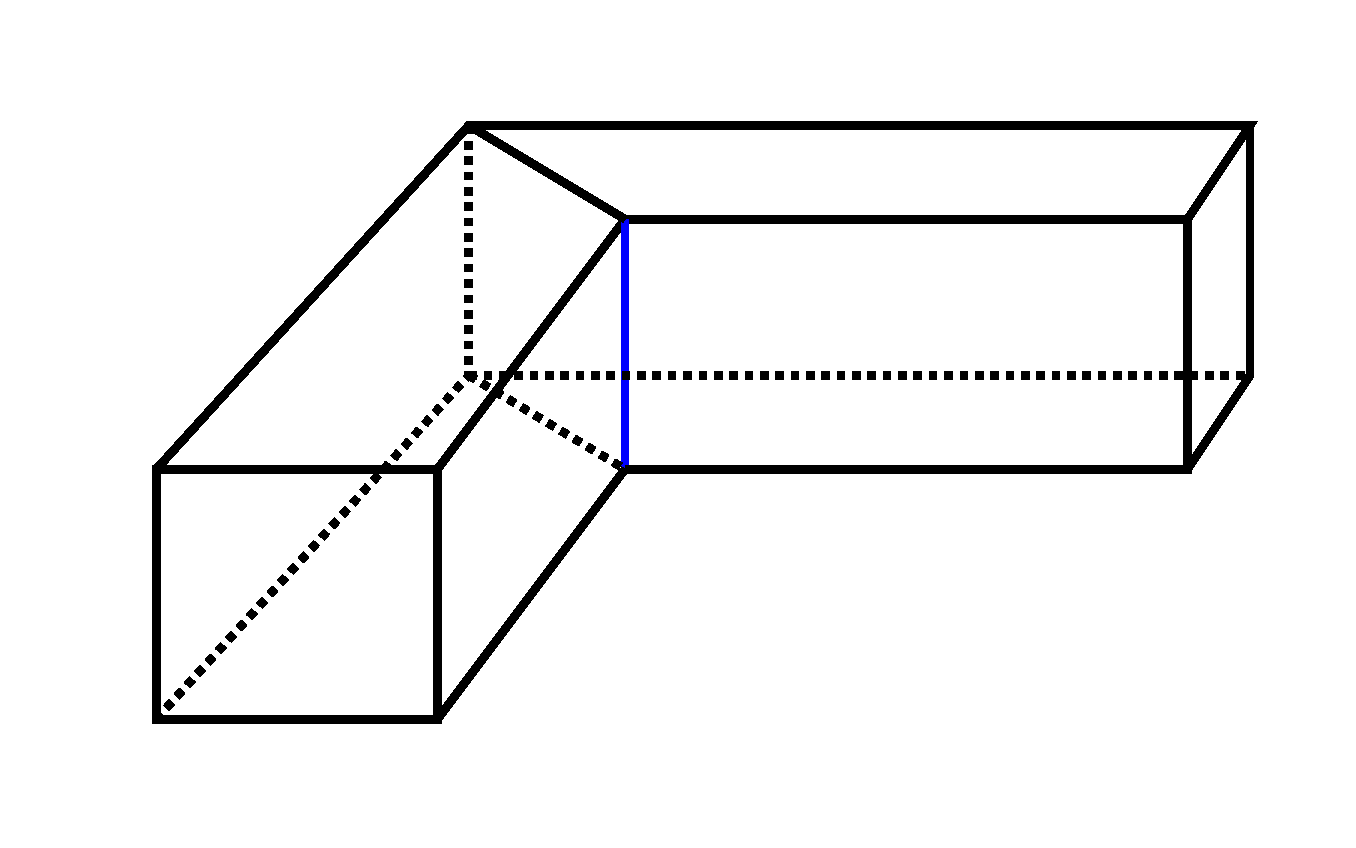
\includegraphics[width=.3\textwidth]{meshes/reflex}
\caption{A polyhedron with one reflex edge (blue), the two vertices incident to the blue
edge are reflex vertices.}
\label{fig:reflex}
\end{figure}


Chazelle and Shouraboura use the 
 Gauss-Bonnet theorem to show that, any polyhedron
 of genus $g$ must have at least $g-1$ reflex edges.
 This implies that any polyhedron
can be triangulated with $O(n+r^2)$ tetrahedra, regardless  of 
the genus! Moreover, the bound is tight \cite{tetra-bounds-c-s-1994}.


Chazell and Palios give an
algorithm to triangulate a nonconvex three-dimensional polyhedra with genus
zero \cite{triangulating-polytope-1990}.
Let $n$ be the number of vertices and $r$ the number of reflex edges,
 their algorithm creates a triangulation with $O(n+r^2)$ tetrahedra 
in $O(n\log r +r^2\log r)$ time and $O(n+r^2)$ space.
Their algorithm first removes $n-4r$ non-reflex or flat vertices
The create a polyhedron with $O(r)$ vertices.
Then, vertical planes decompose the reduced polyhedra in to
$O(r^2)$ convex cells.
In the worst case, decomposing a polyhedron of genus
zero into convex parts requires $\Omega(n^2)$ convex pieces
\cite{chazelle-lower-1984}.
Thus, the algorithm summarized above is tight.


For a genus $g$ polyhedron, it is natural to ask if one can 
triangulate the manifold with fewer than $O(n+r^2)$ tetrahedra.
We now show how Gauss-Bonnet theorem is used to give a negative answer 
 \cite{tetra-bounds-c-s-1994}.
We first show a bound on the number of reflex edges
in a surface of genus $g$.


\begin{theorem}[Reflex Angles]\label{thm:reflex}

Any polyhedron of genus $g$ must have 
at least $g-1$ reflex dihedral angles. 

\end{theorem}

From \thmref{reflex}, it follows that any polyhedron
with $n$ vertices and $r$ reflex angles
can be triangulated with $O(n+r^2)$ tetrahedra 
and the bound is tight. Notice that this result is independent
of the genus.

Let $T$ be a tetrahedra, here, the curvature at a vertex $k_v$ is defined to
be the sum of the angle defect.
The Euler characteristic of a polyhedron is determined by the genus,
$\chi=2-2g$.
Polyhedra do not have a 1-dimensional boundary, 
so, the Gauss-Bonnet theorem,
$$\sum_vk_v=2\pi (2-2g).$$

We show that
$$g\leq r+1.$$ 
Then, \thmref{reflex} will be a consequence of the following
lemma,

\begin{lemma}\label{lem:reflex-edge}
The number of reflex edges  incident to a vertex $v$  is at least $-k_v.$
\end{lemma}

\begin{proof}

Project the faces incident to $v$ onto a 2-sphere centered at $v$
to obtain a ``polygon" $P$on the sphere made  of great circles.
An edge in $T$ is reflex if and only if it gives  a reflex angle on $P$.

Let $L$ be the length of the curve and $R$ is  number of reflex  angles.
Then

\begin{equation} \label{eqn:length-reflex}
L\leq 2\pi (R+1)
\end{equation}
Note, if $R$ is zero then \eqnref{length-reflex}
tells us that the curvature at a convex point is non-negative.

If $R\neq 0$, we draw arcs of great circles from each reflex point
along the bisector of its reflex angle, and thus decompose the unit sphere
into at most $R+1$ convex regions. (Convex here means
great circles are contained in the region).
Apply the $R=0$ case $R+1$ times.

\end{proof}

\begin{figure}[htb]
        \centering
        \begin{subfigure}[b]{0.25\textwidth}
        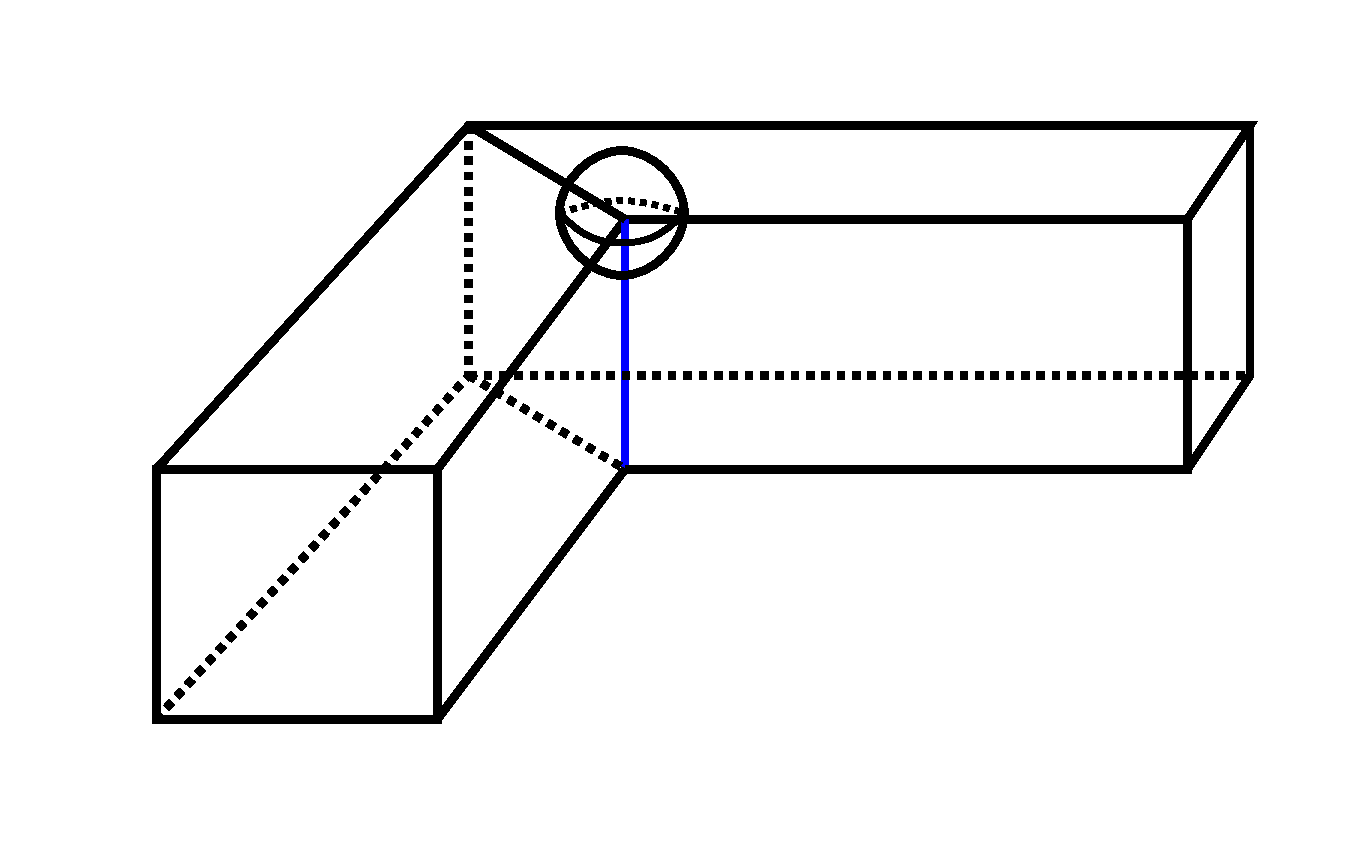
\includegraphics[width=\textwidth]{meshes/reflex-vert-sphere}
        \caption{}
          \label{fig:sphere-on-vert}
        \end{subfigure}
          \hspace{.0cm}
         \begin{subfigure}[b]{0.25\textwidth}
        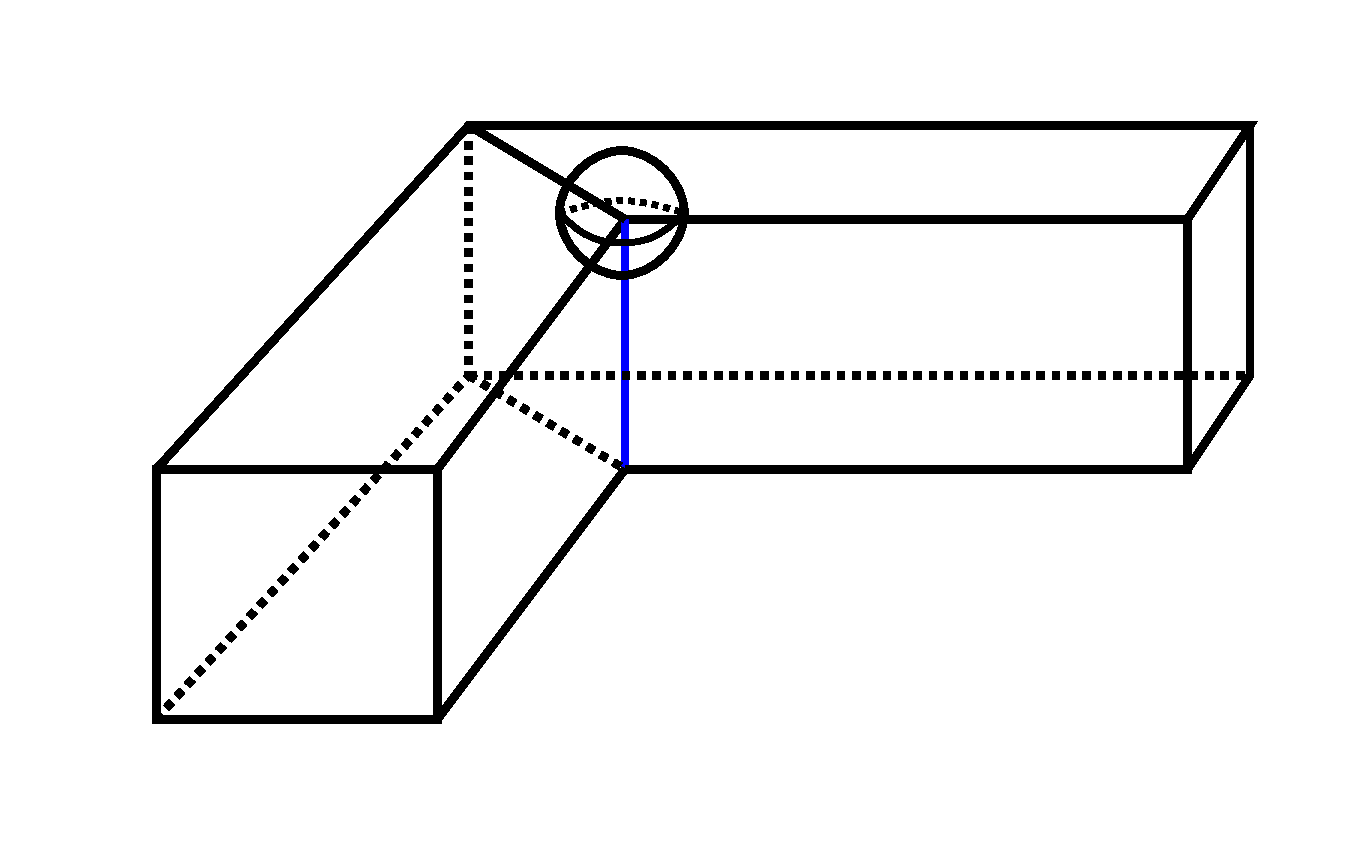
\includegraphics[width=\textwidth]{meshes/reflex-vert-sphere}
        \caption{}
        \label{fig:sphere}
        \end{subfigure}\\
		\caption{(a) A sphere around a reflex vertex. (b) The surface
		intersecting the sphere.
		\label{fig:sphere}}
\end{figure}


